% Created 2018-11-19 lun 12:04
% Intended LaTeX compiler: pdflatex
\documentclass[xcolor={usenames,svgnames,dvipsnames}]{beamer}
\usepackage[utf8]{inputenc}
\usepackage[T1]{fontenc}
\usepackage{graphicx}
\usepackage{grffile}
\usepackage{longtable}
\usepackage{wrapfig}
\usepackage{rotating}
\usepackage[normalem]{ulem}
\usepackage{amsmath}
\usepackage{textcomp}
\usepackage{amssymb}
\usepackage{capt-of}
\usepackage{hyperref}
\usepackage{color}
\usepackage{listings}
\usepackage{mathpazo}
\usepackage{gensymb}
\usepackage{amsmath}
\usepackage{esdiff}
\usepackage{steinmetz}
\bibliographystyle{plain}
\AtBeginSubsection[]{\begin{frame}[plain]\tableofcontents[currentsubsection,sectionstyle=show/shaded,subsectionstyle=show/shaded/hide]\end{frame}}
\AtBeginSection[]{\begin{frame}[plain]\tableofcontents[currentsection,hideallsubsections]\end{frame}}
\usepackage[emulate=units]{siunitx}
\sisetup{fraction=nice, decimalsymbol=comma, retain-unity-mantissa = false}
\newunit{\wattpeak}{Wp}
\newunit{\watthour}{Wh}
\newunit{\amperehour}{Ah}
\hypersetup{colorlinks=true, linkcolor=Blue, urlcolor=Blue}
\renewcommand{\thefootnote}{\fnsymbol{footnote}}
\beamertemplatenavigationsymbolsempty
\setbeamertemplate{footline}[frame number]
\newcommand{\laplace}[1]{\mathbf{#1}(\mathbf{s})}
\newcommand{\slp}{\mathbf{s}}
\newcommand{\fasor}[1]{\mathbf{#1}(\omega)}
\newcommand{\atan}{\mathrm{atan}}
\setbeamercolor{alerted text}{fg=blue!50!black} \setbeamerfont{alerted text}{series=\bfseries}
\usetheme[hideothersubsections]{Goettingen}
\usecolortheme{rose}
\usefonttheme{serif}
\author{Oscar Perpiñán Lamigueiro}
\date{Octubre 2018}
\title{Análisis del Régimen Transitorio con Variables de Estado}
\subtitle{Teoría de Circuitos III}
\hypersetup{
 pdfauthor={Oscar Perpiñán Lamigueiro},
 pdftitle={Análisis del Régimen Transitorio con Variables de Estado},
 pdfkeywords={},
 pdfsubject={},
 pdfcreator={Emacs 25.2.2 (Org mode 9.1.13)}, 
 pdflang={Spanish}}
\begin{document}

\maketitle

\section{Introducción}
\label{sec:orgfe890f6}
\begin{frame}[label={sec:org92e8a4e}]{Motivación}
El comportamiento de un circuito puede ser descrito con ecuaciones diferenciales que pueden ser reescritas a un sistema de ecuaciones de primer orden\footnote{Notación: \[\dot{x} = \diff{x(t)}{t}\]}:

\begin{align*}
  \dot{x}_1 &= \left[a_{11} x_1(t) + \dots + a_{1n} x_n(t)\right] + \left[b_{11} u_1(t) + \dots + b_{1m}u_r(t) \right]\\
  \vdots\\
    \dot{x}_n &= \left[a_{n1} x_1(t) + \dots + a_{nn} x_n(t)\right] + \left[b_{n1} u_1(t) + \dots + b_{nr}u_r(t) \right] 
\end{align*}

\begin{align*}
  y_1(t) &= \left[c_{11} x_1(t) + \dots + c_{1n} x_n(t)\right] + \left[d_{11} u_1(t) + \dots + d_{1r}u_r(t) \right]\\
  \vdots\\
    y_m(t) &= \left[c_{m1} x_1(t) + \dots + c_{mn} x_n(t)\right] + \left[d_{m1} u_1(t) + \dots + d_{mr}u_r(t) \right] 
\end{align*}
\end{frame}

\begin{frame}[label={sec:org8e1269b}]{Nomenclatura}
\begin{itemize}
\item \(x_1(t) \dots x_n(t)\) son las \alert{n} variables del circuito, denominadas \alert{variables de estado}, representadas como un vector \(\mathbf{x}\) de dimensión n (\alert{vector de estado})
\begin{itemize}
\item \emph{Elegimos tensiones de condensadores y corrientes de bobinas}.
\end{itemize}
\end{itemize}
\pause
\begin{itemize}
\item \(u_1(t) \dots u_r(t)\) son las \alert{r} entradas del circuito, representadas con un vector \(\mathbf{u}\) de dimensión r (\alert{vector de entrada})
\end{itemize}
\pause
\begin{itemize}
\item \(y_1(t) \dots y_m(t)\) son las \alert{m} salidas del circuito, representadas con un vector \(\mathbf{y}\) de dimensión m (\alert{vector de salida})
\end{itemize}
\end{frame}


\begin{frame}[label={sec:orgde0bade}]{Notación funcional y matricial}
\begin{block}{Ecuación de estado}
\begin{align*}
\dot{\mathbf{x}} &= f(\mathbf{x}, \mathbf{u}, t)\\
\dot{\mathbf{x}} &= \mathbf{A}\mathbf{x} + \mathbf{B}\mathbf{u}\\
\end{align*}
\end{block}

\begin{block}{Ecuación de salida\footnote{Frecuentemente la matriz \(\mathbf{D}\) es nula, \(\mathbf{y} = \mathbf{C}\mathbf{x}\).}}
\begin{align*}
\mathbf{y} &= g(\mathbf{x}, \mathbf{u}, t)\\
\mathbf{y} &= \mathbf{C}\mathbf{x} + \mathbf{D}\mathbf{u} 
\end{align*}
\end{block}
\end{frame}

\begin{frame}[label={sec:org14d9953}]{Diagrama de Bloques}
\begin{center}
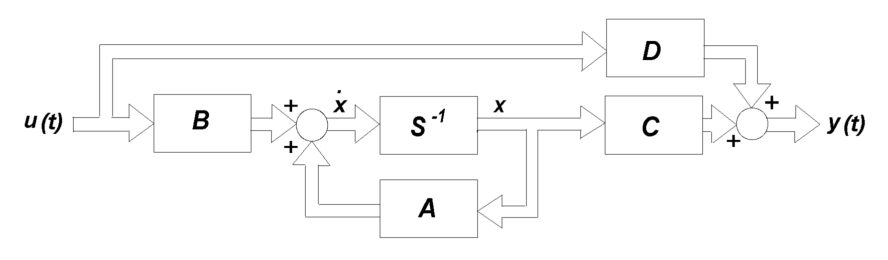
\includegraphics[width=.9\linewidth]{../figs/Bloques_Variables_Estado.pdf}
\end{center}

\begin{align*}
  \dot{\mathbf{x}} &= \mathbf{A}\mathbf{x} + \mathbf{B}\mathbf{u}\\
  \mathbf{y} &= \mathbf{C}\mathbf{x} + \mathbf{D}\mathbf{u} 
\end{align*}
\end{frame}

\begin{frame}[label={sec:orgdbae9ac}]{Ventajas del análisis con variables de estado}
\begin{itemize}
\item Las ecuaciones diferenciales son de primer orden. Existen numerosas técnicas disponibles para resolverlas.
\item Ecuaciones de estado y de salida se pueden programar fácilmente (\emph{enfoque orientado a computación}).
\item Teoría de Sistemas: amplio conocimiento matemático para determinar las propiedades de la solución.
\end{itemize}
\end{frame}

\begin{frame}[label={sec:org5815dda}]{Trayectoria}
\begin{itemize}
\item Supongamos un circuito de segundo orden determinado por las variables \(i_L(t)\) y \(v_c(t)\).
\item La \alert{evolución con el tiempo} de estas dos variables (\emph{intercambio y disipación de energía almacenada}) se puede representar como \alert{coordenadas de puntos en un plano}.
\item El plano \(i_L\) -- \(v_C\) es el \alert{espacio de estados}. La curva que une estos puntos es la \alert{trayectoria en el espacio de estados}.
\item La curva comenzará en el punto de condiciones iniciales, \([i_L(0^+), v_C(0^+)]\), y finalizará en el régimen permanente \([i_L(\infty), v_C(\infty)]\).
\end{itemize}
\end{frame}

\begin{frame}[label={sec:org3944265}]{Trayectoria}
\begin{center}
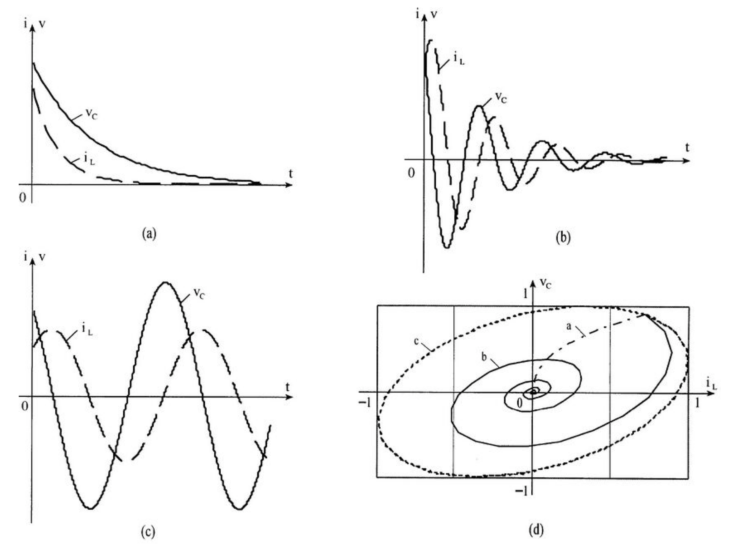
\includegraphics[width=.9\linewidth]{../figs/trayectoria.pdf}
\end{center}
\end{frame}

\section{Topología de Redes}
\label{sec:orge3732b2}

\begin{frame}[label={sec:org4daf473}]{Definiciones}
\begin{itemize}
\item \alert{Grafo}: representación simplificada de un circuito eléctrico.
\end{itemize}

\begin{center}
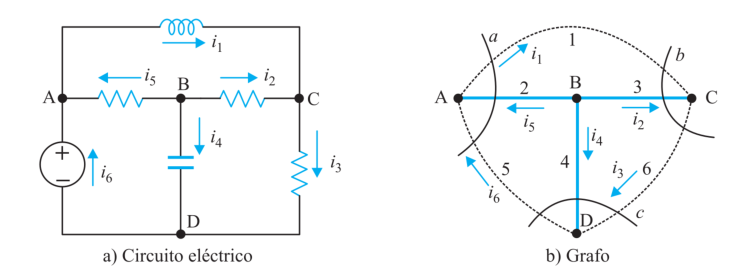
\includegraphics[width=.9\linewidth]{../figs/grafo.pdf}
\end{center}
\end{frame}

\begin{frame}[label={sec:org59955f3}]{Definiciones}
\begin{itemize}
\item \alert{Árbol}: conjunto de ramas que unen todos los nudos sin formar caminos cerrados.
\end{itemize}

\begin{center}
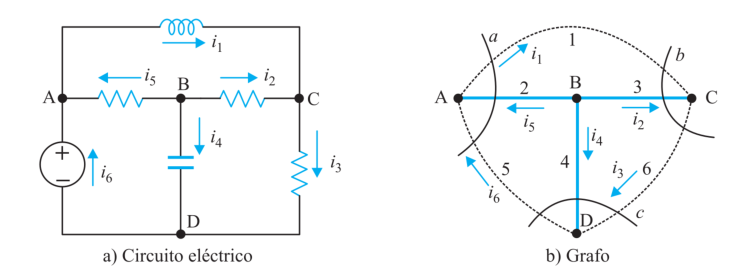
\includegraphics[width=.9\linewidth]{../figs/grafo.pdf}
\end{center}
\end{frame}

\begin{frame}[label={sec:org01dd49b}]{Definiciones}
\begin{itemize}
\item \alert{Cuerdas} o \alert{Eslabones}: ramas no incluidas en el árbol.
\item \alert{Lazos básicos}: lazos de un árbol con sólo un eslabón.
\end{itemize}
\begin{center}
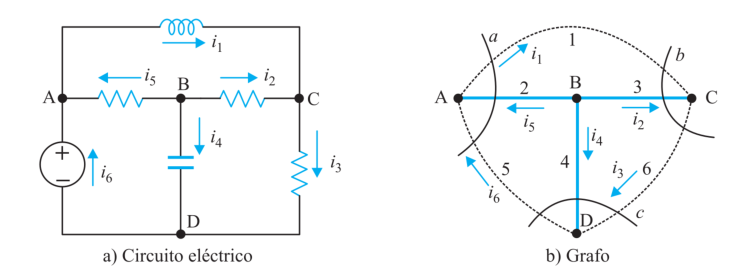
\includegraphics[width=.9\linewidth]{../figs/grafo.pdf}
\end{center}
\end{frame}

\begin{frame}[label={sec:org168f77f}]{Definiciones}
\begin{itemize}
\item \alert{Grupos de corte}: conjunto de ramas al que aplica la LKC.
\item \alert{Grupos de corte básicos}: grupo de corte que contiene sólo una rama del árbol.
\end{itemize}

\begin{center}
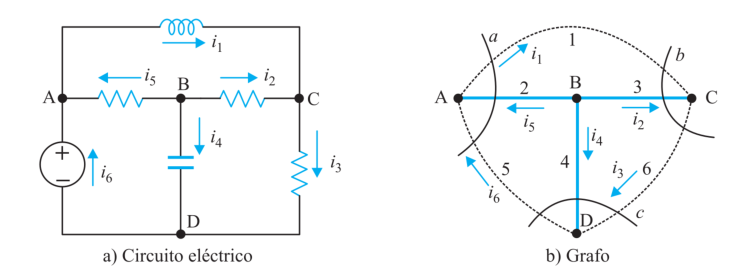
\includegraphics[width=.9\linewidth]{../figs/grafo.pdf}
\end{center}
\end{frame}

\begin{frame}[label={sec:org690298e}]{LKC y LKV}
\begin{itemize}
\item Al aplicar la \alert{LKC} en los \alert{grupos de corte básico} se obtienen ecuaciones linealmente independientes.
\item Al aplicar la \alert{LKV} en los \alert{lazos básicos} se obtienen ecuaciones linealmente independientes.
\end{itemize}
\end{frame}

\section{Planteamiento Sistemático de Ecuaciones}
\label{sec:org0f7ffda}

\begin{frame}[label={sec:org9d5507a}]{Árbol Propio}
\begin{block}{Fundamento}
\begin{itemize}
\item Las variables de estado a elegir son \(u_C(t)\) e \(i_L(t)\).
\item Las ecuaciones de condensadores evalúan corrientes (LKC en grupos de corte básico).
\end{itemize}
\[
\diff{u_c}{t} = \frac{i_c}{C}
\] 
\begin{itemize}
\item Las ecuaciones de bobinas evalúan tensiones (LKV en lazos básicos)
\end{itemize}
\[
\diff{i_L}{t} = \frac{u_L}{L}
\] 
\end{block}
\end{frame}

\begin{frame}[label={sec:org7bab74f}]{Árbol propio}
\begin{block}{Composición}
\begin{itemize}
\item Todas las fuentes de tensión.
\item Todos los condensadores.
\item Resistencias (las que sean necesarias).
\item Ninguna inductancia (situar en eslabones).
\item Ninguna fuente de corriente (situar en eslabones).
\end{itemize}
\end{block}
\end{frame}

\begin{frame}[label={sec:org911da04}]{Ecuación de estado en forma normal}
\begin{enumerate}
\item Establecer el \alert{árbol normal}.\pause
\item \alert{Variables de Estado}: asignar tensiones (\emph{con polaridad}) a condensadores y corrientes (\emph{con sentido}) a inductancias.\pause
\item \alert{Variables adicionales}: tensiones y corrientes en resistencias según necesidad.\pause
\item Una \alert{ecuación para cada condensador} (usando LKC en el grupo de corte básico que corresponda).\pause
\item Una \alert{ecuación para cada inductancia} (usando LKV en el lazo básico que corresponda).\pause
\item \alert{Ecuaciones para resistencias} para determinar variables adicionales (punto 3) en función de variables de estado.\pause

\item Usar ecuaciones de punto 6 en puntos 4 y 5
\end{enumerate}
\end{frame}

\section{Resolución}
\label{sec:org00ca7b6}

\begin{frame}[label={sec:orgecedebc}]{Laplace}
\begin{block}{Ecuación de Estado}
\begin{align*}
  \dot{\mathbf{x}} &= \mathbf{A}\mathbf{x} + \mathbf{B}\mathbf{u}\\
  \slp \laplace{X} - \mathbf{x}(0^-) &= \mathbf{A}\laplace{X} + \mathbf{B}\laplace{U}\\
\end{align*}
\end{block}
\begin{block}{Ecuación de Salida}
\begin{align*}
  \mathbf{y} &= \mathbf{C}\mathbf{x}\\
  \laplace{Y} &= \mathbf{C}\laplace{X}
\end{align*}
\end{block}
\end{frame}
\begin{frame}[label={sec:orga994ed8}]{Ecuación de Estado con Laplace}
\begin{block}{Desarrollo}
\begin{align*}
  \slp \laplace{X} - \mathbf{x}(0^-) &= \mathbf{A}\laplace{X} + \mathbf{B}\laplace{U}\\
  \slp \laplace{X} - \mathbf{A}\laplace{X} &= \mathbf{x}(0^-) + \mathbf{B}\laplace{U}\\
  \left(\slp \mathbf{I} - \mathbf{A} \right) \laplace{X} &= \mathbf{x}(0^-) + \mathbf{B}\laplace{U}\\
  \laplace{X} &= \left(\slp \mathbf{I} - \mathbf{A} \right)^{-1} \mathbf{x}(0^-) +\\ 
  &+ \left(\slp \mathbf{I} - \mathbf{A} \right)^{-1} \mathbf{B}\laplace{U}
\end{align*}
\end{block}
\end{frame}

\begin{frame}[label={sec:org7b05701}]{Matriz \(\slp \mathbf{I} - \mathbf{A}\)}
\[
\slp \mathbf{I} - \mathbf{A} = 
\begin{bmatrix} 
\slp - a_{11} & -a_{12} & \dots & -a_{1n}\\
- a_{21} & \slp -a_{22} & \dots & -a_{2n}\\
\vdots & \vdots & \dots & \vdots \\
- a_{n1} & -a_{n2} & \dots & \slp - a_{nn}
\end{bmatrix}
\]

\[
\left(\slp \mathbf{I} - \mathbf{A} \right)^{-1} = \frac{\text{adj}(\slp \mathbf{I} - \mathbf{A})^T}{\det(\slp \mathbf{I} - \mathbf{A})}
\]
\end{frame}

\begin{frame}[label={sec:orga0ca4f5}]{Solución de la Ecuación de Estado}
\begin{block}{Solución}
\[
  \laplace{X} = \left(\slp \mathbf{I} - \mathbf{A} \right)^{-1} \mathbf{x}(0^-) + \left(\slp \mathbf{I} - \mathbf{A} \right)^{-1} \mathbf{B}\laplace{U}
\]
\end{block}

\begin{block}{Respuesta a Entrada Cero}
\[
  \left(\slp \mathbf{I} - \mathbf{A} \right)^{-1} \mathbf{x}(0^-)
\]
\end{block}

\begin{block}{Respuesta a Estado Inicial Cero}
\[
  \left(\slp \mathbf{I} - \mathbf{A} \right)^{-1} \mathbf{B}\laplace{U}
\]
\end{block}
\end{frame}

\begin{frame}[label={sec:org7e69ebd}]{Función de Transferencia}
\begin{block}{Función de Transferencia}
Suponiendo condiciones iniciales nulas:
\begin{align*}
  \laplace{X} &= \left(\slp \mathbf{I} - \mathbf{A} \right)^{-1} \mathbf{B} \laplace{U}\\
  \laplace{Y} &= \mathbf{C} \laplace{X}\\
  \laplace{H} &= \frac{\laplace{Y}}{\laplace{U}}  = \mathbf{C} \left(\slp \mathbf{I} - \mathbf{A} \right)^{-1} \mathbf{B}
\end{align*}
\end{block}

\begin{block}{Polos del Sistema}
\[
  \left(\slp \mathbf{I} - \mathbf{A} \right)^{-1} = \frac{\text{adj}(\slp \mathbf{I} - \mathbf{A})^T}{\det(\slp \mathbf{I} - \mathbf{A})}
\]
Los polos del sistema se calculan con:
\[
|\slp \mathbf{I} - \mathbf{A}| = 0
\]
\end{block}
\end{frame}
\section{Ejercicios Recomendados}
\label{sec:orgc7186a2}

\begin{frame}[label={sec:org4ed8ce1}]{Ejercicios}
\begin{itemize}
\item FM: Ejemplo de aplicación 4.18
\item HKD: Ejemplos 19.1, 19.2, 19.3
\item Exámenes
\end{itemize}
\end{frame}
\end{document}